
%% bare_conf.tex
%% V1.3
%% 2007/01/11
%% by Michael Shell
%% See:
%% http://www.michaelshell.org/
%% for current contact information.
%%
%% This is a skeleton file demonstrating the use of IEEEtran.cls
%% (requires IEEEtran.cls version 1.7 or later) with an IEEE conference paper.
%%
%% Support sites:
%% http://www.michaelshell.org/tex/ieeetran/
%% http://www.ctan.org/tex-archive/macros/latex/contrib/IEEEtran/
%% and
%% http://www.ieee.org/

%%*************************************************************************
%% Legal Notice:
%% This code is offered as-is without any warranty either expressed or
%% implied; without even the implied warranty of MERCHANTABILITY or
%% FITNESS FOR A PARTICULAR PURPOSE! 
%% User assumes all risk.
%% In no event shall IEEE or any contributor to this code ber liable for
%% any damages or losses, including, but not limited to, incidental,
%% consequential, or any other damages, resulting from the use or misuse
%% of any information contained here.
%%
%% All comments are the opinions of their respective authors and are not
%% necessarily endorsed by the IEEE.
%%
%% This work is distributed under the LaTeX Project Public License (LPPL)
%% ( http://www.latex-project.org/ ) version 1.3, and may be freely used,
%% distributed and modified. A copy of the LPPL, version 1.3, is included
%% in the base LaTeX documentation of all distributions of LaTeX released
%% 2003/12/01 or later.
%% Retain all contribution notices and credits.
%% ** Modified files should be clearly indicated as such, including  **
%% ** renaming them and changing author support contact information. **
%%
%% File list of work: IEEEtran.cls, IEEEtran_HOWTO.pdf, bare_adv.tex,
%%                    bare_conf.tex, bare_jrnl.tex, bare_jrnl_compsoc.tex
%%*************************************************************************

% *** Authors should verify (and, if needed, correct) their LaTeX system  ***
% *** with the testflow diagnostic prior to trusting their LaTeX platform ***
% *** with production work. IEEE's font choices can trigger bugs that do  ***
% *** not appear when using other class files.                            ***
% The testflow support page is at:
% http://www.michaelshell.org/tex/testflow/



% Note that the a4paper option is mainly intended so that authors in
% countries using A4 can easily print to A4 and see how their papers will
% look in print - the typesetting of the document will not typically be
% affected with changes in paper size (but the bottom and side margins will).
% Use the testflow package mentioned above to verify correct handling of
% both paper sizes by the user's LaTeX system.
%
% Also note that the "draftcls" or "draftclsnofoot", not "draft", option
% should be used if it is desired that the figures are to be displayed in
% draft mode.
%
\documentclass[conference]{IEEEtran}

%\usepackage[latin1]{inputenc}
\usepackage{graphicx}
\usepackage[spanish]{babel}
\usepackage[utf8]{inputenc}
\usepackage[FIGTOPCAP]{subfigure}
\usepackage{verbatim}
\usepackage{amsmath}
\usepackage{textcomp}
\usepackage{amssymb}
\usepackage{amsfonts}
\usepackage[normalem]{ulem}
\usepackage{multirow}
\usepackage{balance}
\usepackage{color}
\usepackage{hyperref}
\usepackage{spverbatim}
\usepackage{longtable}
\usepackage[table]{xcolor}


\newtheorem{theorem}{Theorem}[section]
\newtheorem{lemma}[theorem]{Lemma}
\newtheorem{proposition}[theorem]{Proposition}
\newtheorem{corollary}[theorem]{Corollary}

\newcommand{\R}{\mathbb{R}}  % Conjunto de n�meros reales
\newcommand{\N}{\mathbb{N}}  % Conjunto de n�meros naturales
\newcommand{\Z}{\mathbb{Z}}  % Conjunto de n�meros enteros
\newcommand{\C}{\mathbb{C}}  % C�digo = conjunto de palabras c�digo
\newcommand{\E}{\mathbb{E}}  % Esperanza Matem�tica
\newcommand{\F}{\mathbb{F}}  % Cuerpo o campo F
\newcommand{\U}{\mathbb{U}}  %
\newcommand{\X}{\mathbb{X}}  %
\newcommand{\Y}{\mathbb{Y}}  %
\newcommand{\G}{\mathbb{G}}  %
\newcommand{\I}{\mathbb{I}}  %

\newcommand{\tab}{\hspace{0.3cm}} % tabulacion

\newcommand{\ScaleA}{1.0} % tabulacion
 
\newcommand{\NC}[2]{%N�mero Combinatorio
\left(\!\!\begin{array}{c}#1\\#2\end{array}\!\!\right)
}

% Use this alternative format:

% Page Layout
%\addtolength{\columnsep}{0mm}         % gap between columns
%\addtolength{\topmargin}{0mm}         % gap above header

\addtolength{\topskip}{-0mm}          % between header and text

\addtolength{\textheight}{1.5mm}        % height of main text

\addtolength{\textwidth}{1.6mm}         % width of text
\addtolength{\oddsidemargin}{-0.8mm}    % odd page left margin

%\addtolength{\evensidemargin}{0mm}    % even page left margin

% Paragraphs
%\addtolength{\parindent}{0mm}         % indentation of paragraphs
%\addtolength{\parskip}{0mm}           % gap between paragraphs

% Floats (tables and figures) 
%\addtolength{\floatsep}{0mm}          % space left between floats.

%\addtolength{\textfloatsep}{-2mm}     % space between last top float or first bottom float and the text.
\addtolength{\textfloatsep}{-2.0mm}    % space between last top float or first bottom float and the text.

%\addtolength{\intextsep}{0mm}         % space left on top and bottom of an in-text float.
%\addtolength{\dbltextfloatsep}{0mm}   % is \textfloatsep for 2 column output.
%\addtolength{\dblfloatsep}{0mm}       % is \floatsep for 2 column output.
\addtolength{\abovecaptionskip}{-0.5mm} % space above caption
\addtolength{\belowcaptionskip}{-0.5mm} % space below caption

% Maths
\addtolength{\abovedisplayskip}{-0.5mm} % space before maths
\addtolength{\belowdisplayskip}{-0.5mm} % space after maths
%\addtolength{\arraycolsep}{0mm}       % gap between columns of an array

% Lists
%\addtolength{\topsep}{0mm}           % space between first item and preceding paragraph.
%\addtolength{\partopsep}{0mm}        % extra space added to \topsep when environment starts a new paragraph.
%\addtolength{\itemsep}{0mm}          % space between successive items.


% Add the compsoc option for Computer Society conferences.
%
% If IEEEtran.cls has not been installed into the LaTeX system files,
% manually specify the path to it like:
% \documentclass[conference]{../sty/IEEEtran}


% Some very useful LaTeX packages include:
% (uncomment the ones you want to load)


% *** MISC UTILITY PACKAGES ***
%
%\usepackage{ifpdf}
% Heiko Oberdiek's ifpdf.sty is very useful if you need conditional
% compilation based on whether the output is pdf or dvi.
% usage:
% \ifpdf
%   % pdf code
% \else
%   % dvi code
% \fi
% The latest version of ifpdf.sty can be obtained from:
% http://www.ctan.org/tex-archive/macros/latex/contrib/oberdiek/
% Also, note that IEEEtran.cls V1.7 and later provides a builtin
% \ifCLASSINFOpdf conditional that works the same way.
% When switching from latex to pdflatex and vice-versa, the compiler may
% have to be run twice to clear warning/error messages.






% *** CITATION PACKAGES ***
%
%\usepackage{cite}
% cite.sty was written by Donald Arseneau
% V1.6 and later of IEEEtran pre-defines the format of the cite.sty package
% \cite{} output to follow that of IEEE. Loading the cite package will
% result in citation numbers being automatically sorted and properly
% "compressed/ranged". e.g., [1], [9], [2], [7], [5], [6] without using
% cite.sty will become [1], [2], [5]--[7], [9] using cite.sty. cite.sty's
% \cite will automatically add leading space, if needed. Use cite.sty's
% noadjust option (cite.sty V3.8 and later) if you want to turn this off.
% cite.sty is already installed on most LaTeX systems. Be sure and use
% version 4.0 (2003-05-27) and later if using hyperref.sty. cite.sty does
% not currently provide for hyperlinked citations.
% The latest version can be obtained at:
% http://www.ctan.org/tex-archive/macros/latex/contrib/cite/
% The documentation is contained in the cite.sty file itself.






% *** GRAPHICS RELATED PACKAGES ***
%
\ifCLASSINFOpdf
  % \usepackage[pdftex]{graphicx}
  % declare the path(s) where your graphic files are
  % \graphicspath{{../pdf/}{../jpeg/}}
  % and their extensions so you won't have to specify these with
  % every instance of \includegraphics
  % \DeclareGraphicsExtensions{.pdf,.jpeg,.png}
\else
  % or other class option (dvipsone, dvipdf, if not using dvips). graphicx
  % will default to the driver specified in the system graphics.cfg if no
  % driver is specified.
  % \usepackage[dvips]{graphicx}
  % declare the path(s) where your graphic files are
  % \graphicspath{{../eps/}}
  % and their extensions so you won't have to specify these with
  % every instance of \includegraphics
  % \DeclareGraphicsExtensions{.eps}
\fi
% graphicx was written by David Carlisle and Sebastian Rahtz. It is
% required if you want graphics, photos, etc. graphicx.sty is already
% installed on most LaTeX systems. The latest version and documentation can
% be obtained at: 
% http://www.ctan.org/tex-archive/macros/latex/required/graphics/
% Another good source of documentation is "Using Imported Graphics in
% LaTeX2e" by Keith Reckdahl which can be found as epslatex.ps or
% epslatex.pdf at: http://www.ctan.org/tex-archive/info/
%
% latex, and pdflatex in dvi mode, support graphics in encapsulated
% postscript (.eps) format. pdflatex in pdf mode supports graphics
% in .pdf, .jpeg, .png and .mps (metapost) formats. Users should ensure
% that all non-photo figures use a vector format (.eps, .pdf, .mps) and
% not a bitmapped formats (.jpeg, .png). IEEE frowns on bitmapped formats
% which can result in "jaggedy"/blurry rendering of lines and letters as
% well as large increases in file sizes.
%
% You can find documentation about the pdfTeX application at:
% http://www.tug.org/applications/pdftex





% *** MATH PACKAGES ***
%
%\usepackage[cmex10]{amsmath}
% A popular package from the American Mathematical Society that provides
% many useful and powerful commands for dealing with mathematics. If using
% it, be sure to load this package with the cmex10 option to ensure that
% only type 1 fonts will utilized at all point sizes. Without this option,
% it is possible that some math symbols, particularly those within
% footnotes, will be rendered in bitmap form which will result in a
% document that can not be IEEE Xplore compliant!
%
% Also, note that the amsmath package sets \interdisplaylinepenalty to 10000
% thus preventing page breaks from occurring within multiline equations. Use:
%\interdisplaylinepenalty=2500
% after loading amsmath to restore such page breaks as IEEEtran.cls normally
% does. amsmath.sty is already installed on most LaTeX systems. The latest
% version and documentation can be obtained at:
% http://www.ctan.org/tex-archive/macros/latex/required/amslatex/math/





% *** SPECIALIZED LIST PACKAGES ***
%
%\usepackage{algorithmic}
% algorithmic.sty was written by Peter Williams and Rogerio Brito.
% This package provides an algorithmic environment fo describing algorithms.
% You can use the algorithmic environment in-text or within a figure
% environment to provide for a floating algorithm. Do NOT use the algorithm
% floating environment provided by algorithm.sty (by the same authors) or
% algorithm2e.sty (by Christophe Fiorio) as IEEE does not use dedicated
% algorithm float types and packages that provide these will not provide
% correct IEEE style captions. The latest version and documentation of
% algorithmic.sty can be obtained at:
% http://www.ctan.org/tex-archive/macros/latex/contrib/algorithms/
% There is also a support site at:
% http://algorithms.berlios.de/index.html
% Also of interest may be the (relatively newer and more customizable)
% algorithmicx.sty package by Szasz Janos:
% http://www.ctan.org/tex-archive/macros/latex/contrib/algorithmicx/




% *** ALIGNMENT PACKAGES ***
%
%\usepackage{array}
% Frank Mittelbach's and David Carlisle's array.sty patches and improves
% the standard LaTeX2e array and tabular environments to provide better
% appearance and additional user controls. As the default LaTeX2e table
% generation code is lacking to the point of almost being broken with
% respect to the quality of the end results, all users are strongly
% advised to use an enhanced (at the very least that provided by array.sty)
% set of table tools. array.sty is already installed on most systems. The
% latest version and documentation can be obtained at:
% http://www.ctan.org/tex-archive/macros/latex/required/tools/


%\usepackage{mdwmath}
%\usepackage{mdwtab}
% Also highly recommended is Mark Wooding's extremely powerful MDW tools,
% especially mdwmath.sty and mdwtab.sty which are used to format equations
% and tables, respectively. The MDWtools set is already installed on most
% LaTeX systems. The lastest version and documentation is available at:
% http://www.ctan.org/tex-archive/macros/latex/contrib/mdwtools/


% IEEEtran contains the IEEEeqnarray family of commands that can be used to
% generate multiline equations as well as matrices, tables, etc., of high
% quality.


%\usepackage{eqparbox}
% Also of notable interest is Scott Pakin's eqparbox package for creating
% (automatically sized) equal width boxes - aka "natural width parboxes".
% Available at:
% http://www.ctan.org/tex-archive/macros/latex/contrib/eqparbox/





% *** SUBFIGURE PACKAGES ***
%\usepackage[tight,footnotesize]{subfigure}
% subfigure.sty was written by Steven Douglas Cochran. This package makes it
% easy to put subfigures in your figures. e.g., "Figure 1a and 1b". For IEEE
% work, it is a good idea to load it with the tight package option to reduce
% the amount of white space around the subfigures. subfigure.sty is already
% installed on most LaTeX systems. The latest version and documentation can
% be obtained at:
% http://www.ctan.org/tex-archive/obsolete/macros/latex/contrib/subfigure/
% subfigure.sty has been superceeded by subfig.sty.



%\usepackage[caption=false]{caption}
%\usepackage[font=footnotesize]{subfig}
% subfig.sty, also written by Steven Douglas Cochran, is the modern
% replacement for subfigure.sty. However, subfig.sty requires and
% automatically loads Axel Sommerfeldt's caption.sty which will override
% IEEEtran.cls handling of captions and this will result in nonIEEE style
% figure/table captions. To prevent this problem, be sure and preload
% caption.sty with its "caption=false" package option. This is will preserve
% IEEEtran.cls handing of captions. Version 1.3 (2005/06/28) and later 
% (recommended due to many improvements over 1.2) of subfig.sty supports
% the caption=false option directly:
%\usepackage[caption=false,font=footnotesize]{subfig}
%
% The latest version and documentation can be obtained at:
% http://www.ctan.org/tex-archive/macros/latex/contrib/subfig/
% The latest version and documentation of caption.sty can be obtained at:
% http://www.ctan.org/tex-archive/macros/latex/contrib/caption/




% *** FLOAT PACKAGES ***
%
%\usepackage{fixltx2e}
% fixltx2e, the successor to the earlier fix2col.sty, was written by
% Frank Mittelbach and David Carlisle. This package corrects a few problems
% in the LaTeX2e kernel, the most notable of which is that in current
% LaTeX2e releases, the ordering of single and double column floats is not
% guaranteed to be preserved. Thus, an unpatched LaTeX2e can allow a
% single column figure to be placed prior to an earlier double column
% figure. The latest version and documentation can be found at:
% http://www.ctan.org/tex-archive/macros/latex/base/



%\usepackage{stfloats}
% stfloats.sty was written by Sigitas Tolusis. This package gives LaTeX2e
% the ability to do double column floats at the bottom of the page as well
% as the top. (e.g., "\begin{figure*}[!b]" is not normally possible in
% LaTeX2e). It also provides a command:
%\fnbelowfloat
% to enable the placement of footnotes below bottom floats (the standard
% LaTeX2e kernel puts them above bottom floats). This is an invasive package
% which rewrites many portions of the LaTeX2e float routines. It may not work
% with other packages that modify the LaTeX2e float routines. The latest
% version and documentation can be obtained at:
% http://www.ctan.org/tex-archive/macros/latex/contrib/sttools/
% Documentation is contained in the stfloats.sty comments as well as in the
% presfull.pdf file. Do not use the stfloats baselinefloat ability as IEEE
% does not allow \baselineskip to stretch. Authors submitting work to the
% IEEE should note that IEEE rarely uses double column equations and
% that authors should try to avoid such use. Do not be tempted to use the
% cuted.sty or midfloat.sty packages (also by Sigitas Tolusis) as IEEE does
% not format its papers in such ways.





% *** PDF, URL AND HYPERLINK PACKAGES ***
%
%\usepackage{url}
% url.sty was written by Donald Arseneau. It provides better support for
% handling and breaking URLs. url.sty is already installed on most LaTeX
% systems. The latest version can be obtained at:
% http://www.ctan.org/tex-archive/macros/latex/contrib/misc/
% Read the url.sty source comments for usage information. Basically,
% \url{my_url_here}.





% *** Do not adjust lengths that control margins, column widths, etc. ***
% *** Do not use packages that alter fonts (such as pslatex).         ***
% There should be no need to do such things with IEEEtran.cls V1.6 and later.
% (Unless specifically asked to do so by the journal or conference you plan
% to submit to, of course. )


% correct bad hyphenation here
\hyphenation{op-tical net-works semi-conduc-tor}


\begin{document}
%
% paper title
% can use linebreaks \\ within to get better formatting as desired

\title{Implementación de un Sistema en Chip con Microprocesador Soft-Core y Soporte Linux/ecOS}

% conference papers do not typically use \thanks and this command
% is locked out in conference mode. If really needed, such as for
% the acknowledgment of grants, issue a \IEEEoverridecommandlockouts
% after \documentclass

% for over three affiliations, or if they all won't fit within the width
% of the page, use this alternative format:
\author{
%\IEEEauthorblockN{Damian A. Morero\IEEEauthorrefmark{1}\IEEEauthorrefmark{2} and Mario R. Hueda\IEEEauthorrefmark{1}}
\IEEEauthorblockN{Valeria Lovaisa Michelini \IEEEauthorrefmark{1} Pablo Roberto Gomez \IEEEauthorrefmark{1} Federico Paredes \IEEEauthorrefmark{1} Orlando Micolini\IEEEauthorrefmark{1}}
 
\IEEEauthorblockA{ \IEEEauthorrefmark{1} Laboratorio de Arquitectura de Computadoras 
  - Universidad Nacional de Córdoba \\ Av. Velez
  Sarsfield 1611 - Córdoba (X5016GCA) - Argentina}

%\IEEEauthorblockA{\IEEEauthorrefmark{2}ClariPhy Argentina S.A. - Humberto Primo 680 - C�rdoba (5000) - Argentina}
}

% use for special paper notices
%\IEEEspecialpapernotice{(Invited Paper)}


% make the title area
\maketitle


\begin{abstract}
%\boldmath 

La eficiencia que demostraron los sistemas embebidos en la solución de problemas específicos produjeron un incremento significativo en su demanda. 

En este trabajo se aborda el análisis y la implementación de dos SoC de código abierto, ambos con núcleo OpenRISC 1200, sobre una placa de desarrollo con soporte para dos sistemas operativos ecOS y Linux, con la finalidad de obtener un sistema integral de código abierto en donde se tiene código HDL, assembler y C disponible para realizar sistemas optimizados para una función especifica.

 Mediante el empleo del modelo de desarrollo en espiral se plantearon una serie de prototipos que incluyeron mayor funcionalidad en cada iteración. Dando lugar en cada prototipo a la prueba del funcionamientos de los distintos modulos de cada SoC implementado sobre la FPGA.

Este proceso tuvo como resultado la instanciación de dos SoC de código abierto sobre la placa de desarrollo de Xilinx S3ADSP1800A, utilizando aproximadamente el 50\% de los recursos en la FPGA para ambos SoC. Para la evaluación del OpenRISC 1200 se ejecutaron los benchmarks de sistemas embebidos Coremark y Dhrystone los resultados fueren para el primero 1.52/MHz y para el segundo 10.53 DMIP. Se observó que para distintos niveles de optimización del compilador cruzado or32-elf-gcc tuvo una mejora temporal y espacial en el código generado.

Los resultados de las benchmark permitieron posicionar al OpenRISC respecto de otros procesadores comerciales. El sistema operativo ecOS se monto con éxito en el SoC mostrando el correcto funcionamiento de manejo de hilos, se compiló exitosamente el kernel de Linux pudiendo comprobarse su correcta implemetación sobre una arquitectura OpenRISC 1200.
 



%Background information
%La reducción de tamaño es el primer paso para la fabricación de biocombustibles a partir de biomasa leñosa. Se lleva a cabo generalmente utilizando máquinas de fresado y el tamaño de partícula se controla por el tamaño del tamiz instalado en una máquina de fresado 
%
%Propósito (tiempo pasado / presente perfecto / presente simple) 
%En este trabajo se aborda el diseño y análisis técnico-económico de un sistema integrado para la producción de biodiesel a partir de aceite de algas producida a través del secuestro de dióxido de carbono de los gases de combustión de una planta de energía.
%
%Metodología (tiempo pasado) 
%"Se utilizó un procedimiento de transesterificación en dos etapas para eliminar los altos contenidos de ácidos grasos libres en el aceite de cocina usado (OMA)." 
%"Ultrasonidos, una técnica de proceso no convencional, se aplicó a convertir directamente el aceite de cocina usado en biodiesel en un solo paso."
%
% Resultados (pueden expresarse en presente simple, pero más comúnmente en pasado simple) 
%"Este proceso dio lugar a una materia prima para biodiesel rendimiento de conversión de aproximadamente el 85-96\%, utilizando un catalizador de sulfato férrico. En el método de transesterificación metanol supercrítico, el rendimiento de biodiésel fue de aproximadamente 50-65\% en sólo 15 minutos de tiempo de reacción ".
%
%Conclusiones (presentar verbos auxiliares provisionales / tiempo / modal) 
%"Los resultados de las pruebas revelaron que el método de proceso supercrítico es probablemente un método alternativo promisorio para el tradicional proceso de transesterificación en dos etapas usando un catalizador de sulfato férrico para los residuos de cocina de conversión de petróleo." 
%"A partir de este resultado, se concluye que la manteca de cerdo de residuos puede ser utilizado como materia prima alternativa para la producción de biodiesel a partir de un proceso supercrítico, sustituyendo así el alto costo refinado materia prima de aceite vegetal."
%
%
%Background
%un número de estudios
%es / se supone que
%está / están basados ​​en
%Se ha demostrado recientemente que ...
%Se sabe que ...
%Es ampliamente aceptado que la ...
%investigación reciente / estudios
%
%objetivo
%Nuestro enfoque ...
%El objetivo de este estudio es ...
%comparar / examinar / investigar / estudio
%
%Metodología / Materiales 
%... Fue o fueron calculadas / construido / evaluado / formulado / medida / modelo / interpretadas / estudio / tratados / usado 
%
%3. Resultados 
%Se observó / observado que ... 
%El resultado fue ... 
%... Fue o fueron alcanzados / identificado / found / obtenida / presente / no afectado (por) 
%  ... Dado ...
%
%4. Aplicaciones 
%se puede aplicar / usado 
%hacer posible 
%uso potencial 
%relevante para / en 
%
%5. Limitaciones y trabajos futuros 
%un intento preliminar 
%futura direcciones / trabajo
\end{abstract}
% IEEEtran.cls defaults to using nonbold math in the Abstract.
% This preserves the distinction between vectors and scalars. However,
% if the conference you are submitting to favors bold math in the abstract,
% then you can use LaTeX's standard command \boldmath at the very start
% of the abstract to achieve this. Many IEEE journals/conferences frown on
% math in the abstract anyway.

% no keywords




% For peer review papers, you can put extra information on the cover
% page as needed:
% \ifCLASSOPTIONpeerreview
% \begin{center} \bfseries EDICS Category: 3-BBND \end{center}
% \fi
%
% For peerreview papers, this IEEEtran command inserts a page break and
% creates the second title. It will be ignored for other modes.
\IEEEpeerreviewmaketitle



%-------------------------------------------------------------------------------------------------
%-------------------------------------------------------------------------------------------------
%-------------------------------------------------------------------------------------------------
\section{Introducción} \label{sec:intro}
Los sistemas embebidos tienen un importante rol en la optimización de soluciones para problemas específicos que van desde un control de temperatura para un acondicionador de aire hasta el sistema de control y el procesamiento de señales en un satélite de
telecomunicaciones. Los criterios de optimización suelen enfocarse en reducir el costo, el consumo y el tamaño de los sistemas.

El presente trabajo muestra una solución descripta en hardware código abierto, sobre una arquitectura OpenRISC 1200 utilizando FPGA, con soporte para los sistemas operativos Linux y ecOs; Tal sistema de código abierto se caracteriza por ser tecnológicamente independiente implementándose tanto a nivel de FPGAs de bajo costo como a nivel de Circuitos Integrados para Aplicaciones Específicas(ASIC). Además con un diseño de código abierto existe la opción de personalizar la descripción RTL
para implementar la optimización o la funcionalidad deseada.


\subsection{Objetivo General}% \label{sec:errorfloor_model}

Implementar un sistema embebido basado en hardware\footnote{Entendiéndose por hardware de código abierto al código Register Transfer Level (RTL)} y software de código abierto.
Dicho hardware será un Sistemas programables en Chip (SoC) montado sobre una placa de desarrollo que deberá además soportar un sistema operativo
libre con la finalidad de proveer un sistema integral FPGA-SoC-Sistema
Operativo completamente funcional de código abierto para aplicaciones de pequeña envergadura.


\subsection{Objetivos específicos}% \label{sec:errorfloor_model}
 \begin{itemize}
 \item Analizar los microprocesadores softcore disponibles y seleccionar el microprocesador que se adapta mejor a nuestros requerimientos.

\item Seleccionar los SoCs de acuerdo al microprocesador softcore elegido y determinar la placa de desarrollo para su implementación.

\item Estudiar y aplicar los mecanismos para la medición del rendimiento de sistemas embebidos. 

\item Estudiar los Sistemas Operativos existentes soportados por las plataformas elegidas.

\item Implementar el flujo de diseño de hardware para cada SoC seleccionado y realizar las correcciones necesarias sobre el código RTL para su correcta implementación. 

\item Poner en funcionamiento y configurar los sistemas operativos Linux y ecOS para los SoCs elegidos.

\item Verificar y validar cada prototipo implementado para la detección de deficiencias del microprocesador, los SoCs, sus módulos y las herramientas de entorno de software para la arquitectura seleccionada.

%\item Desarrollar  aplicaciones en lenguaje C generadas mediante compilación cruzada para las pruebas del funcionamiento del microprocesador, los SoCs, sus modulos y las herramientas de entorno de software para la arquitectura seleccionada.

%\item Presentar los Sistemas Operativos Linux y eCos que poseen las prestaciones funcionales adecuadas para su utilización en Sistemas Embebidos.

 \end{itemize}

%1-establecer la importancia de su campo proporcionan hechos fondo / información (posiblemente desde la investigación) definir la terminología en el título / palabras claves presentan el área del problema / enfoque de la investigación actual
%
%2-investigación y las contribuciones anteriores y / o actuales 
%
%3-encontrar una brecha en la investigación a describir el problema que se dirigirá a la actualidad una predicción a ensayar 
%
%4-describir el presente trabajo

\section{Marco Teórico} %\label{sec:background}

\subsection{Field Programmable Gate Arrays (FPGAs)}% \label{sec:errorfloor_model}
Son circuitos integrados formados por bloques lógicos 
programables e interconectables entre sí. Permiten 
implementar sistemas de alta complejidad y flexibilidad, 
pudiendo combinarse con periféricos y microprocesadores; 
para formar los llamados «Sistemas programables en chip».


\subsection{Intellectual Property Core (IP Core) }% \label{sec:errorfloor_model}

El diseño de circuitos digitales se divide en bloques
funcionales que se denominan \textit{módulos} o \textit{cores}. Un
\textit{core} puede influir un conjunto de sub-bloques que ayudan a
poner en práctica su funcionalidad. Los \textit{cores} pueden variar
en tamaño partiendo de la implementación de una simple operación
aritmética hasta la implementación de un microprocesador completo. El
mismo \textit{core} puede ocupar una FPGA entera conformando el
producto final completo o puede ser simplemente un bloque entre otros
en una FPGA más grande o en un ASIC. Los \textit{cores} generalmente se describen utilizando un Lenguaje de Descripción de Hardware (HDL)
en un nivel de abstracción conocida como Register Transfer Level
(RTL).

A los cores pueden diseñarlos una persona o una entidad. Los
desarrolladores de \textit{cores} y licenciatarios varían desde
particulares a empresas. El producto, en este caso se conoce como un
\textit{IP core (Intellectual Property Core)} siendo el diseño la
propiedad intelectual de los desarrolladores.

Pueden clasificarse de la siguiente manera:
 \begin{itemize}
\item{Softcores} Son los más flexibles y se presentan para \textit{IP}
  en forma netlist (lista de compuertas e interconexiones) o en forma
  de sintetizable RTL, lo que los hace tecnológicamente
  independientes. Los \textit{cores} sintetizables se entregan en un
  lenguaje de descripción de hardware como Verilog o VHDL. Para utilizarse en diferentes aplicaciones, pero poseen una menor
  predictibilidad en la implementación y suelen tener un mayor costo y
  menor desempeño de procesamiento.

\item{Firmcores} Estos cores están optimizados para
  implementarse en una FPGA, arquitectura o dispositivo en
  particular. Esta optimización puede realizarla el fabricante
  o un tercero. Utilizar este tipo de IP-Cores requiere disponer
  de cierto nivel de conocimiento de la arquitectura, ya que es
  posible rutear señales físicas y especificar la colocación de los
  elementos de diseño. Un ejemplo de estos cores es el procesador
  MicroBlaze de Xilinx~\cite{Etiqueta04}

\item{Hardcores} Están optimizados para una tecnología específica y el diseñador que los utiliza no puede modificarlos. Son
  manifestaciones físicas del diseño del core ya que tienen un layout
  predefinido incluido en la arquitectura. Son los mejores para
  aplicaciones plug\&play. Si bien son poco flexibles, portables y
  configurables, son muy predictibles (timing fijo) y fiables
  una vez implementados.
\end{itemize}

\subsection{Microprocesadores Soft Core}% \label{sec:errorfloor_model}

Es un microprocesador que puede implementarse utilizando síntesis lógica
en diferentes dispositivos lógicos programables. Particularmente destacados por su alto nivel de configuración, pudiendo agregar y quitar funcionalidades en base a las 
necesidades específicas \cite{Etiqueta22} Suelen distribuirse en forma de código fuente en algún lenguaje de descripción de hardware, principalmente VHDL o Verilog, aunque algunos comerciales se distribuyen en formatos propietarios.

El microprocesador como componente discreto o como parte en un mismo 
chip, es un buen candidato para ser implementado en un FPGA. Esto implica, que el microprocesador se encargue de la ejecución de programas secuenciales y cálculos; mientras que la lógica de la FPGA se encarga de las interfaces, además de facilitar el procesamiento paralelo. En cuanto a performance, varía respecto a cada implementación, dependiendo de las características inherentes a la CPU, como tipos y tamaños de cache, buses, controladores, etc. ~\cite{Etiqueta05}.

	Los principales fabricantes de dispositivos lógicos programables, tienen su propio Soft Core comercial diseñado y optimizado para funcionar en sus FPGAs. También existe una gran variedad de distribuidos en forma de código abierto, como el OpenRISC 1200 \cite{Etiqueta19} mantenido por la comunidad Opencores \cite{Etiqueta20}, o los  SCPs
	LEON2 y LEON3 \cite{Etiqueta21} \cite{Etiqueta22} que proporciona la compañía Gaisler Research \cite{Etiqueta23}.



\subsection{Benchmarking}% \label{sec:errorfloor_model}

Es una forma de medir el rendimiento de un sistema o los componentes del mismo. Se obtiene por la acción de ejecutar un programa de computadora o un conjunto de programas. Dicho rendimiento se refiere generalmente al hardware.Sin embargo, hay circunstancias en que la técnica también es aplicable al software

El uso de \textit{benchmark} está motivado por la creciente
complejidad en los sistemas informáticos, tanto a nivel de hardware
como de software, lo cual dificulta enormemente su comparación. En
particular, las especificaciones técnicas del sistema por sí solas no
permiten predecir el rendimiento del mismo para resolver un problema
en particular. Es necesario utilizar tests que permitan su
comparación.

Entre la amplia variedad de \textit{benchmarks} existentes podemos
diferenciar dos grupos principales. El primer grupo lo conforman los
\textit{benchmarks} de aplicaciones los cuales se encargan de analizar
el rendimiento cuando se ejecutan programas de uso cotidiano para el
usuario. El segundo grupo lo conforman los \textit{benchmarks}
sintéticos diseñados para imitar una clase particular
de carga de trabajo en un componente del sistema. Estos últimos son
más efectivos para probar componentes individuales como discos rígidos
o dispositivos de red.

La utilización de benchmarking se extiende a los Sistemas Embebidos
proporcionando datos que permiten la comparación de los mismos. Por
ejemplo, el Embedded Microprocessor Benchmark Consortium (EEMBC)
desarrolla una serie de aplicaciones benchmark que facilitan a los
diseñadores de sistemas la selección de los procesadores óptimos para
sus desarrollos. EEMBC organiza su conjunto de benchmarks apuntando a
diferentes ramas de aplicación tales como Automotriz, Sistemas
Digitales, Java, Procesadores Multicore, Redes, Procesamiento de
señales, Smartphones/tablets y Browsers.
	
En benchmarking de sistema embebidos es común realizar tests que se
focalicen en el núcleo de la CPU aislándolo de los otros elementos del
procesador. Es posible, por ejemplo, que desee tener la capacidad de
hacer caso omiso de la memoria y los efectos de E/S con el fin de
focalizar el análisis principalmente en la operación de un pipeline.

A continuación se describen dos de los principales benchmarks que se
utilizaron para evaluar el sistema desarrollado en el trabajo presente
CoreMark es un Benchmark que pretende medir el desempeño de las CPU
utilizadas en Sistemas Embebidos. Fue desarrollado en 2009 por Shay
Gal-On en el EEMBC y se ha convertido en un estándar de la
industria, llegando a reemplazar al antiguo benchmark
Dhrystone. CoreMark esta desarrollado en C y contiene implementaciones
de los siguientes algoritmos:
	
\begin{itemize}
\item Procesamiento de listas (Find and sort)
\item Manipulación de matrices (Operaciones comunes de matrices)
\item Máquina de estados 
\item Códigos de redundancia cíclica (CRC)  
\end{itemize}	 
	
Las plataformas actuales con procesadores embebidos no solo están
compuestas por un CPU y un subsistema de memoria. De hecho, los SoC
pueden estar compuestos por más de un núcleo de CPU, aceleradores de
hardware, periféricos complejos y grandes cantidades de
memoria. CoreMark es el punto de partida para la evaluación de éstos
complejos dispositivos. El benchmark es capaz de probar la estructura
de pipeline básica de un procesador, así como la capacidad de prueba
de lectura/escritura de operaciones básicas, operaciones de enteros y
operaciones de control. Respecto de los periféricos y mecanismos de
interrupción, el EEMBC desarrolla una colección de tests basados en
escenarios y conducidos por hardware que evalúan dichos periféricos
y la capacidad del CPU de prestar servicio a los mismos y a otras
interrupciones a nivel sistema.
	
Los resultados del CoreMark pueden verse en la página principal   
del proyecto \url{http://www.eembc.org/coremark/}

\subsection{Dhrystone}

 		Es un benchmark sintético y comercial. Intenta medir la velocidad del sistema en cuanto a rendimiento no numérico, expresando los
		resultados en DPS (instrucciones Dhrystones Por Segundo). El rendimiento de Dhyrstone se calcula a partir de la siguiente fórmula: Iteraciones
		Dhrystone por segundo = reloj del procesador * número de pasadas / tiempo de ejecución. Para que el resultado sea válido, el código Dhrystone debe
		ejecutarse al menos por dos segundos. %Es un pequeño benchmark sintético que pretende ser representativo de programación entera de sistemas. 
		
		Contiene muchas instrucciones simples, llamadas a procedimiento y condicionales, y pocas de coma flotante y bucles. Usa pocas variables globales y
		ejecuta operaciones con punteros. Está compuesto por 12 procedimientos incluidos en un bucle de medida con 94 sentencias. No se puede variar su
		tamaño. Está compuesto por un 53\% de instrucciones de asignación, 32\% de instrucciones de control y un 15\% de llamadas a procedimiento.
		Dhrystone es compacto (no más de 1,5 KB), ampliamente disponible en el dominio público, y sencillo de ejecutar. Por ser tan pequeño, Dhrystone
		entra completamente en la caché interna, de esta manera no mide el resto del sistema pero presenta la ventaja de que mide solamente la capacidad
		del procesador para trabajar con enteros.
%-------------------------------------------------------------------------------------------------
%-------------------------------------------------------------------------------------------------
%-------------------------------------------------------------------------------------------------
\section{Métodos y Materiales} \label{sec:background}

\subsection{Metodología}

El modelo de desarrollo a utilizar es el \textit{Modelo en Espiral}. Dicho modelo fue tipificado por Ian Sommerville~\cite{Etiqueta00} y originalmente propuesto por Boehm en
año 1988 en el artículo ``A Spiral Model of Software Development and Enhancement''.
Las fases metodológicas utilizadas para el desarrollo están representados en la Figura 1: 

\begin{figure}[t] 
  \centerline{\includegraphics[width=\ScaleA\columnwidth]{figures_sources/espiral_paper}}%
    \caption{Ciclo de vida de los prototipos}
    \label{fig:pro3enc} 
\end{figure}


Como primer paso se analizarán las diferentes
alternativas disponibles en el mercado y en comunidades de hardware de
código abierto para la implementación de microprocesadores diseñados
en lenguaje de descripción de hardware. Como segundo paso 
se analizarán y seleccionarán los componentes \footnote{Entiéndase como ``componente'' a microprocesadores softcore, SoC, placa de desarrollo.} por medio de un análisis comparativo que permitirá evidenciar las características relevantes de
cada uno de ellos. Como último paso debido a que se adoptara un modelo de desarrollo en espiral se plantearán una serie de prototipos que incluirán mayor funcionalidad en cada iteración del modelo.

\subsection{Recursos Utilizados}

La implementación del sistema se llevó a cabo sobre la placa de
desarrollo de Xilinx S3ADSP1800A, basada en hardware reconfigurable disponible en
el Centro Universitario de Automatización y Robótica (CUDAR) de la
Universidad Tecnológica Nacional (UTN) de Córdoba. Sin embargo, cabe
destacar que el sistema propuesto puede ser implementado cualquier
otra FPGA que disponga de los recursos mínimos necesarios.

%-------------------------------------------------------------------------------------------------
\section{Desarrollo} %\label{sec:proposed_scheme}
Como primera acción se analizó la factibilidad de implementación de un SoC con licencia OpenSource en FPGA.
\subsection{Requerimientos de Usuario}% \label{sec:numerical_results}
\begin{itemize}
\item Se debe implementar un Microprocesador Softcore de núcleo simple.
\item El SoC seleccionado debe poseer la menor cantidad de restricciones respecto de su implementación en placas de desarrollo de diversos fabricantes.
\item Todo el codigo RTL implementado, las herramientas de desarrollo utilizadas para el diseño de software y los sistemas operativos debe tener licencia LGPL o GPL.
\item
\end{itemize}

\begin{figure}[t] 
  \centerline{\includegraphics[width=\ScaleA\columnwidth]{figures_sources/proto1}}%
    \caption{Ciclo de vida de los prototipos}
    \label{fig:pro3enc} 
\end{figure}

\begin{figure}[t] 
  \centerline{\includegraphics[width=\ScaleA\columnwidth]{figures_sources/proto2}}%
    \caption{Ciclo de vida de los prototipos}
    \label{fig:pro3enc} 
\end{figure}

\begin{figure}[t] 
  \centerline{\includegraphics[width=\ScaleA\columnwidth]{figures_sources/ecos}}%
    \caption{Ciclo de vida de los prototipos}
    \label{fig:pro3enc} 
\end{figure}

\begin{figure}[t] 
  \centerline{\includegraphics[width=\ScaleA\columnwidth]{figures_sources/proto4}}%
    \caption{Ciclo de vida de los prototipos}
    \label{fig:pro3enc} 
\end{figure}

%-------------------------------------------------------------------------------------------------
\subsection{Análisis de Riesgo} %\label{sec:performance_proposed_scheme}



%-------------------------------------------------------------------------------------------------
%\subsection{Example 1} \label{sec:numerical_results}
%
%\begin{table*}[t]
%\caption{\label{tab:examples} Performance and complexity comparison of Example~1.}
%  \begin{center}
%    \begin{tabular}{|c|c|r|c|l|c|c|c|} %\cline{2-4} \multicolumn{1}{c|}{}
%      \multicolumn{1}{c}{Scheme}& 
%      \multicolumn{1}{c}{SNR Penalty}&
%      \multicolumn{1}{c}{Overhead}&
%      \multicolumn{1}{c}{Error Floor}&
%      \multicolumn{1}{c}{Outer Code $\C_2$}&
%      \multicolumn{1}{c}{Outer Code $\C_3$}& 
%      \multicolumn{1}{c}{Performance}&
%      \multicolumn{1}{c}{Complexity}\\ 
%      \hline 
%      SCC-I       & 0.3386 dB   &  8.1081 \%       & None                      & BCH$[1320,1221,19]$    & None                    & Bad   & Good   \\
%      \hline 
%      SCC-II       & 0.0397 dB   &  0.9174 \%       & $\approx 5\cdot 10^{-19}$  & BCH$[47520,47088,55]$  & None     
%      & Good  & Bad    \\
%      \hline 
%      This work         & 0.0297 dB   &  0.6865 \%       & $\approx 5\cdot 10^{-19}$  & RS$[432,396,37]$       & BCH$[1410,1311,19]$  & Good  & Good   \\
%      \hline 
%    \end{tabular}
%    \vspace{-5mm}
%  \end{center}
%\end{table*}
%
%\begin{itemize}
%\item SCC-I: the outer code $\C_2$ must be the
%  BCH$[1320,1221,19]$. Therefore, the SNR penalty and bandwidth
%  overhead are $10\cdot log_{10}(1320/1221)=0.3386$~dB and
%  $(1320-1221)/1221= 8.11\%$, respectively.
%\item SCC-II: the outer code $\C_2$ must be a binary
%  BCH$[47520,47088,55]$ code, which corrects up to $\tau=3$
%  error-patterns of $9$ bits. The error floor is not entirely
%  eliminated, but it is reduced to $P_b^{(I\!I)}(\Omega)\approx 5\cdot
%  10^{-19}$ with an SNR penalty and bandwidth overhead of $0.0397$~dB
%  and $0.9174\%$, respectively.
%\item New SCC: setting $m=36$ and $\tau=3$ as in SCC-II (this way, the
%  same residual error floor is achieved), $\C_3$ can be a
%  BCH$[1410,1311,19]$ over GF$(2^{11})$, and $\C_2$ can be an
%  RS$[432,396,37]$ over GF($2^{9}$). The number of additional parity
%  bits is $36\cdot 9=324$. This OH introduces an SNR penalty and a
%  bandwidth overhead of $0.0297$~dB and $0.6865\%$, respectively.
%\end{itemize}
% 
%Table~\ref{tab:examples} presents a comparison of the different SCC
%solutions. Note that
%\begin{itemize}
%\item the performance of SCC-II is better than that of SCC-I at the
%  expense of a higher implementation complexity (due to the longer
%  outer BCH code);
%\item the new approach achieves better performance than SCC-II with a
%  complexity similar to that of SCC-I\footnote{In particular, note
%    that the outer BCH code of the new SCC and the outer BCH code of
%    SCC-I belong to the same primitive BCH code over GF($2^{11}$)
%    (they have practically the same complexity). Also notice that the
%    second outer RS code of the new SCC is simple and requires only
%    one decoding process per frame.}.
%%\footnote{Also note that since only $\binom{m}{\tau}$
%%    different erasure patterns have to be corrected by $\C_2$, its
%%    decoder could be optimized to lower complexity}.
%\end{itemize}
%
%
%\subsection{Example 2} 
%We use the proposed SCC to improve the performance of the LDPC+RS
%concatenation scheme designed for next generation optical
%communication systems \cite{4528592}. This scheme comprises an inner
%LDPC$[9252,7967]$ code and an outer RS$[992,956,37]$ code. The total
%overhead is $20.5\%$ and the NCG at BER=$10^{-15}$ is $10$~dB. The
%outer RS code introduces an SNR penalty of $0.1605$~dB.
%
%Next we use the new SCC approach with the same inner LDPC code
%$\C_1$. For the outer codes, we consider the RS$[833,797,37]$ as
%$\C_3$ (a shortened version of the original RS code), and the
%RS$[1014,936,79]$ code as $\C_2$ where $m=26$ and $\tau=2$.  From
%\cite{4528592}, the error pattern probability is $P_w(\Omega)\approx
%5\cdot 10^{-7}$. Then, the residual error floor is
%$P_b^{(I\!I\!I)}(\Omega)\approx 10^{-19}$. The SNR penalty and
%bandwidth overhead are $0.0164$~dB and $0.378\%$
%respectively. Finally, we get NCG$=10.1441$~dB (vs. $10$~dB) with a
%total overhead of $16.568\%$ (vs. $20.5\%$).


%-------------------------------------------------------------------------------------------------
%-------------------------------------------------------------------------------------------------
%-------------------------------------------------------------------------------------------------
\section{MEDICIONES} \label{sec:improvements}

\begin{figure}[t] 
  \centerline{\includegraphics[width=\ScaleA\columnwidth]{figures_sources/calculomatriz}}%
    \caption{Ciclo de vida de los prototipos}
    \label{fig:pro3enc} 
\end{figure}


%We introduce two improvements of the new SCC suitable for many
%practical applications based on LDPC codes and TCs. The first one is
%an optimization for $\tau=1$ motivated by the fact that most LDPC
%codes have a low error floor (BER$<10^{-10}$) that can be reduced
%below $10^{-15}$ by correcting only one error pattern per frame (i.e.,
%$\tau=1$). The second approach is a generalization of the SCC
%technique designed to reduce the error floor caused by low-weight
%codewords (i.e., undetectable error patterns). This is particularly
%useful to lower the error floor of TC such as TPC.
%
%\subsection{New SCC with $\tau=1$} \label{sec:improvement_1}
%
%When $\tau=1$ it is possible to lower the overhead penalty,
%implementation complexity, and encoder latency by using ${(n_3-k_3)}$
%\textit{single parity check} (SPC) codes as the outer code $\C_2$. The
%new encoding process, as depicted in Fig.~\ref{fig:pro2enc}, comprises
%the following steps:
%\begin{itemize}
%\item[1.] The uncoded frame is divided into $m$ blocks. The first
%  $m-1$ datawords $D^i_3$ for $i=1,\ldots,m-1$ correspond to the first
%  $m-1$ blocks. The last dataword $D^m_3$ is the concatenation of
%  $(n_3-k_3)$ zeros and the last block $\widetilde{D}^m_3$ of
%  $k_3-(n_3-k_3)$ bits.
%\item[2.] Each dataword $D^i_3$ is encoded by $\C_3$ generating the
%  parity bits $P^i_3$.
%\item[3.] For $i=1,\ldots,n_3-k_3$ the $m$-bit dataword $D^i_2$ is the
%  concatenation of the $i$-th parity bit of $P^j_3$ for
%  $j=1,\ldots,m$. Each $D^i_2$ is encoded by an SPC code.
%\item[4.] The dataword for $\C_1$ is $D^i_1=D^i_3$ for
%  $i=1,\ldots,m-1$. The last dataword $D^m_1$ is the concatenation of
%  $\widetilde{D}^m_3$ and the $n_3-k_3$ parity bits generated in
%  Step~3. Finally, each dataword $D^i_1$ is encoded by $\C_1$.
%\end{itemize}
%
%\begin{figure}[t]
%  \centerline{\includegraphics[width=\ScaleA\columnwidth]{figures_sources/drawing_v10_proposed_2_encoder.eps}}%
%  \caption{Encoding process of the new SCC optimized for $\tau=1$.}
%    \label{fig:pro2enc}
%\end{figure}

% \begin{figure}[t]
%   \centerline{\includegraphics[width=\ScaleA\columnwidth]{figures_sources/drawing_v10_proposed_2_decoder.eps}}%
%     \caption{Decoding process of the SCC optimized for $\tau=1$}
%     \label{fig:pro2dec} 
% \end{figure}

% Figure~\ref{fig:pro2dec} shows an example for the particular
% case in which the error pattern takes place in the codeword $C_1^3$. 
%
%The decoding process is similar to that of the original scheme (e.g.,
%see Fig.~\ref{fig:pro1dec}). The main benefits of this optimized
%scheme are:
%\begin{itemize}
%\item The implementation complexity of the encoder and decoder of the
%  outer code $\C_2$ is very low since they can be implemented with
%  $n_3-k_3$ XOR gates of $m$ input bits.
%\item It is possible to show that the overhead penalty is reduced to
%  $\Theta^{(I\!I\!I)}(1) =
%  \frac{1}{m}\left[\frac{n_3-k_3}{k_3}\right]$ because the corrupted
%  parity-bits of $\C_2$ do not have to be erased.
%\item The latency is reduced because the $P_2^i$ parity bits are
%  transmitted in the last codeword of $\C_1$ (i.e., the parity bits
%  can be computed while the codewords of $\C_1$ are being transmitted).
%\end{itemize}
%
%\begin{figure}[t]
%  \centerline{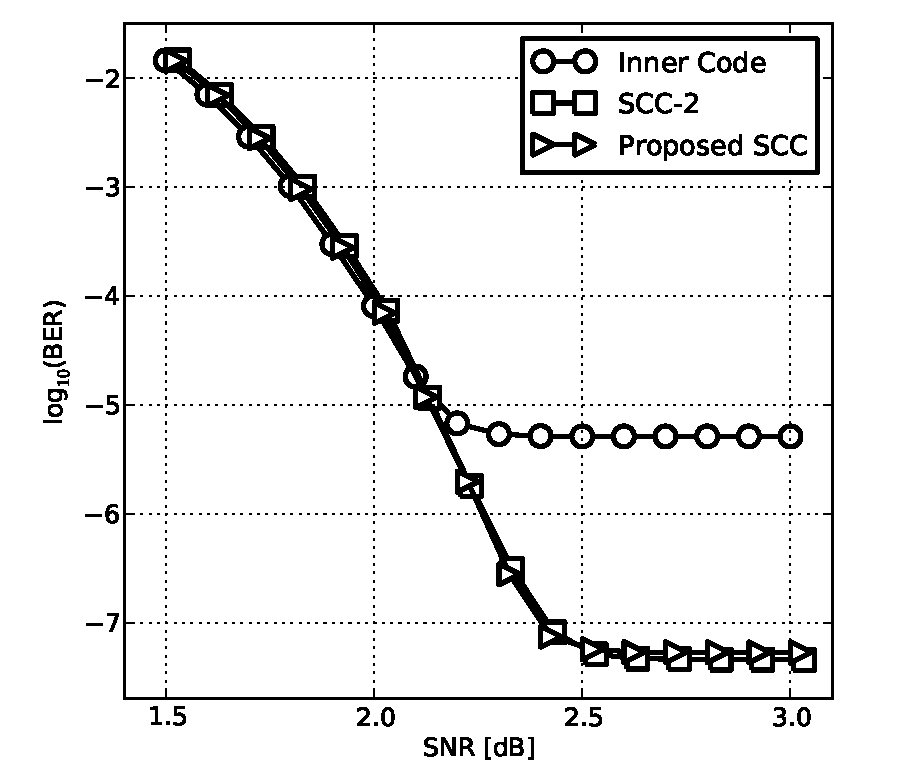
\includegraphics[width=\ScaleA\columnwidth]{figures_sources/BER_vs_SNR_Margulis_with_Scheme1.eps}}%
%  \caption{BER vs SNR for SCC-II and the new SCC with $\tau=1$.}
%    \label{fig:sim1}
%\end{figure}
%
%The performance of the improved SCC approach with $m=10$ is verified
%by using computer simulations in Fig.~\ref{fig:sim1}. The Margulis
%$[2640,1320]$ code is used as inner code, $\C_1$. Owing to time
%constraints, an artificial high error floor with probability
%$P_w(\Omega)=10^{-3}$ is inserted after the decoding
%process. Similarly to the \emph{real} error floor, the artifical BER
%is generated from error patterns with 7 information bits and 7 parity
%bits. Figure~\ref{fig:sim1} shows the BER of the inner code $\C_1$
%(circles), SCC-II (squares) and the proposed SCC (triangles). For
%SCC-II, the outer code $\C_2$ is a BCH$[13200,13102,15]$. On the other
%hand, $\C_3$ is a BCH$[1397,1320,15]$ while $\C_2$ is an
%SPC$[11,10,2]$ code for the new SCC. From Fig.~\ref{fig:sim1} note
%that $\C_1$ has an error floor at
%BER~$\approx\frac{7}{1320}P_w(\Omega) = 5.3\cdot 10^{-6}$. This error
%floor is reduced by the outer codes to BER~$\approx 4.73\cdot
%10^{-8}$. From this figure we see that the new SCC is able to achieve
%a similar performance than SCC-II. It is important to realize that our
%technique achieves this performance by using short outer block
%codes. Compared with SCC-II, this fact reduces significantly the
%implementation complexity in integrated circuits.
% 
%%-------------------------------------------------------------------------------------------------
%\subsection{Generalization to Correct Low-Weight Codewords} \label{sec:proposed_scheme2}
%
%The proposed SCC strategy can be generalized to reduce also the error
%floor due to low-weight codewords (i.e. undetectable error patterns),
%which is particularly useful for turbo codes. Figure~\ref{fig:pro3enc}
%shows the encoding process of the generalized SCC. Unlike the previous
%case, a subset of the parity bits $P^i_3$ of $\C_3$, denoted as
%$\hat{P}^i_3$, is not encoded by $\C_2$. Instead, this subset is
%transmitted as a part of the dataword $D^i_1$ of the inner code
%$\C_1$. In the decoding process, $\hat{P}^i_3$ is used to detect the
%corrupted $\C_1$-codewords. The decoding process starts by applying
%the decoder of code $\C_1$ to the $m$ received codewords
%$C_1^i$. After that, the dataword $D_1^i$ is extracted from
%$C_1^i$. For each dataword $D^i_1$, the dataword $D^i_3$ is extracted
%and \textit{partially} encoded with $\C_3$ in order to regenerate only
%the parity bits $\hat{P}^i_3$. If these regenerated parity bits are
%not equal to the corresponding bits in $D^i_1$, this dataword is
%marked as corrupted. Once all corrupted datawords $D^i_1$ are
%identified, the rest of the decoding process continues as in the
%original SCC.
%
%\begin{figure}[t] 
%  \centerline{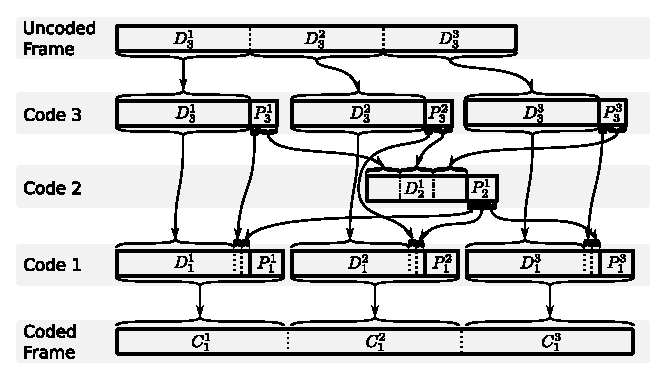
\includegraphics[width=\ScaleA\columnwidth]{figures_sources/drawing_v10_proposed_3_encoder.eps}}%
%    \caption{Encoding process of the generalized SCC.}
%    \label{fig:pro3enc} 
%\end{figure}

%-------------------------------------------------------------------------------------------------
%-------------------------------------------------------------------------------------------------
%-------------------------------------------------------------------------------------------------
\section{CONCLUSIÓN} \label{sec:concl} 

%We have introduced a novel SCC scheme to combat the error floor
%problem experienced in iterated sparse graph-based error correcting
%codes. This SCC scheme is built upon two short outer codes combined
%with a novel encoding/decoding strategy. We have shown that the new
%approach reduces significantly the complexity with negligible
%penalty. The proposed SCC can be efficiently used to combat the error
%floor experienced in both LDPC and TP codes. In particular, the new
%SCC approach can be used to improve the performance in high-speed
%optical communications, where high coding gain and very low BER are
%required.




 
% Note that IEEE typically puts floats only at the top, even when this
% results in a large percentage of a column being occupied by floats.


% An example of a double column floating figure using two subfigures.
% (The subfig.sty package must be loaded for this to work.)
% The subfigure \label commands are set within each subfloat command, the
% \label for the overall figure must come after \caption.
% \hfil must be used as a separator to get equal spacing.
% The subfigure.sty package works much the same way, except \subfigure is
% used instead of \subfloat.
%
%\begin{figure*}[!t]
%\centerline{\subfloat[Case I]\includegraphics[width=2.5in]{subfigcase1}%
%\label{fig_first_case}}
%\hfil
%\subfloat[Case II]{\includegraphics[width=2.5in]{subfigcase2}%
%\label{fig_second_case}}}
%\caption{Simulation results}
%\label{fig_sim}
%\end{figure*}
%
% Note that often IEEE papers with subfigures do not employ subfigure
% captions (using the optional argument to \subfloat), but instead will
% reference/describe all of them (a), (b), etc., within the main caption.


% An example of a floating table. Note that, for IEEE style tables, the 
% \caption command should come BEFORE the table. Table text will default to
% \footnotesize as IEEE normally uses this smaller font for tables.
% The \label must come after \caption as always.
%
%\begin{table}[!t]
%% increase table row spacing, adjust to taste
%\renewcommand{\arraystretch}{1.3}
% if using array.sty, it might be a good idea to tweak the value of
% \extrarowheight as needed to properly center the text within the cells
%\caption{An Example of a Table}
%\label{table_example}
%\centering
%% Some packages, such as MDW tools, offer better commands for making tables
%% than the plain LaTeX2e tabular which is used here.
%\begin{tabular}{|c||c|}
%\hline
%One & Two\\
%\hline
%Three & Four\\
%\hline
%\end{tabular}
%\end{table}


% Note that IEEE does not put floats in the very first column - or typically
% anywhere on the first page for that matter. Also, in-text middle ("here")
% positioning is not used. Most IEEE journals/conferences use top floats
% exclusively. Note that, LaTeX2e, unlike IEEE journals/conferences, places
% footnotes above bottom floats. This can be corrected via the \fnbelowfloat
% command of the stfloats package.








% trigger a \newpage just before the given reference
% number - used to balance the columns on the last page
% adjust value as needed - may need to be readjusted if
% the document is modified later
%\IEEEtriggeratref{8}
% The "triggered" command can be changed if desired:
%\IEEEtriggercmd{\enlargethispage{-5in}}

% references section

% can use a bibliography generated by BibTeX as a .bbl file
% BibTeX documentation can be easily obtained at:
% http://www.ctan.org/tex-archive/biblio/bibtex/contrib/doc/
% The IEEEtran BibTeX style support page is at:
% http://www.michaelshell.org/tex/ieeetran/bibtex/

\bibliographystyle{IEEEtran}

% argument is your BibTeX string definitions and bibliography database(s)
\bibliography{IEEEabrv,paper}

%
% <OR> manually copy in the resultant .bbl file
% set second argument of \begin to the number of references
% (used to reserve space for the reference number labels box)
% \begin{thebibliography}{1}
% 
% \bibitem{IEEEhowto:kopka}
% H.~Kopka and P.~W. Daly, \emph{A Guide to \LaTeX}, 3rd~ed.\hskip 1em plus
%   0.5em minus 0.4em\relax Harlow, England: Addison-Wesley, 1999.
% 
% \end{thebibliography}

\balance


% that's all folks
\end{document}


